% - - - - - - - - - - - - - - - - - - - - - - - - - - - - 
\subsection{PROCM-02 Contratar Nuevo Personal}

\begin{figure}[htbp]
	\begin{center}
		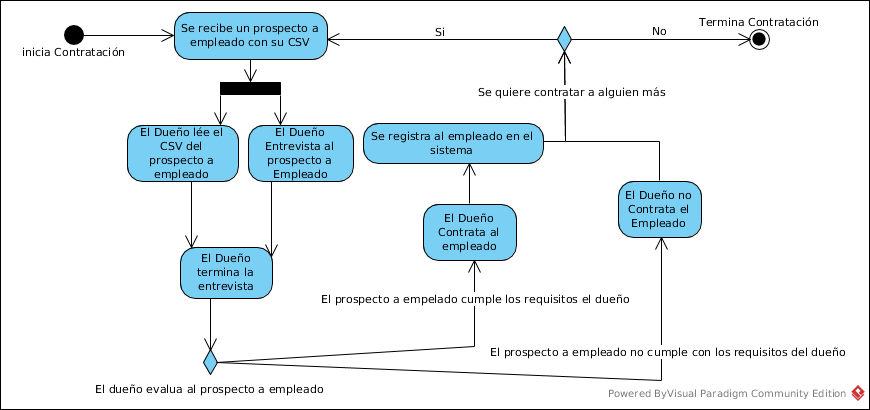
\includegraphics[width=.8\textwidth]{images/TOBEprocContratacion}
		\caption{PROCM-02 Contratar Nuevo Personal}
		\label{fig:proceso3}
	\end{center}
\end{figure}

\begin{description}
	\item[Descripción:]Cuando se abre una nueva sucursal o simplemente se esta escaso de personal, se procede a la contratación del nuevo, dicha contratación es llevada a cabo por el dueño, con el sistema en funcionamiento se espera que se tenga un mejor manejo de los nuevos empleados en la sucursal, así como facilitar la asignación del personal en una sucursal.
	\item[Entradas:] \cdtEmpty
        \begin{itemize}
			\item Datos del nuevo empleado
        \end{itemize}
	\item[Salidas:] \cdtEmpty
        \begin{itemize}
			\item Contrato
        \end{itemize}	
    \item[Mejoras esperadas:] se espera que ahora se pueda tener un mejor control de los empleados..
    \item[Casos de uso:]CU 8 Agregar Empleado.
\end{description}
